\documentclass[presentation]{beamer}
\usetheme{CambridgeUS}
\setbeamertemplate{navigation symbols}{}
\usepackage{tikz,pgf}
\usepackage{threeparttable}%tableNotes
\usepackage{colortbl}%rowcolor
\usepackage{calligra}%Thank You Font
\usepackage{mathtools}
\usepackage{multirow}
\usepackage{amssymb}
\usepackage{listings}
\usepackage{tcolorbox}
\usepackage{xcolor}
\usepackage[T1]{fontenc}
\usetikzlibrary{shapes,arrows,chains,calc,trees,backgrounds,fit,decorations.markings,automata,positioning}
\lstset{%
  basicstyle = \linespread{1.1}\ttfamily\scriptsize,
  tabsize          = 2,     % tab space width
  numbers          = left,  % display line numbers on the left
  commentstyle     = \color{blue},      % comment color
  keywordstyle     = \color{red},       % keyword color
  keywords=[2]{assert},
  stringstyle      = \color{DarkRed},    % string color
  showstringspaces = false, 
  escapechar=!,             % do not mark spaces in strings
  keywordstyle=[2]{\color{blue!80!black}},
  xleftmargin=.05\textwidth
}
\definecolor{green}{rgb}{0.01, 0.7, 0.01}
\definecolor{bole}{rgb}{0.47, 0.27, 0.23}
\definecolor{boston}{rgb}{0.8, 0.0, 0.0}
\definecolor{prune}{rgb}{0.44, 0.11, 0.11}
\setbeamertemplate{headline}{}

\tikzset{onslide/.code args={<#1>#2}{%
		\only<#1>{\pgfkeysalso{#2}} % \pgfkeysalso doesn't change the path
}}
\tikzset{temporal/.code args={<#1>#2#3#4}{%
		\temporal<#1>{\pgfkeysalso{#2}}{\pgfkeysalso{#3}}{\pgfkeysalso{#4}} % \pgfkeysalso doesn't change the path
}}
\tikzstyle{invisible}=[opacity=0,text opacity=0]
\tikzstyle{fvisible}=[opacity=1,text opacity=1]
\tikzstyle{semivisible}=[opacity=0.2,text opacity=0.2]

\newtcbox{\xmybox}[1][blue]{on line,
	arc=1pt,colback=#1!10!white,colframe=#1,
	before upper={\rule[0pt]{0pt}{0pt}},boxrule=1pt,
	boxsep=0pt,left=0pt,right=0pt,top=0pt,bottom=0pt}

%%%%%%%%%%%%%%%%%%%%%%%%%%%%%%%%%%%%%%%%%%%%%%%%%%%%%%%%%%%%%%%%%%%%%%%%%%%%%%%
\title[VLSID 2019]{Improving Performance of a Path-Based
Equivalence Checker using Counter-Examples}
\author[{R. Chouksey et al.}]{\rmfamily Ramanuj Chouksey, Chandan Karfa, and Purandar Bhaduri}
\institute[IIT Guwahati]{Indian Institute of Technology Guwahati}
\date[\tiny\today]{\tiny\today}

\begin{document}
\begin{frame}
\titlepage
\end{frame}

\begin{frame}{Outline}
\tableofcontents
\end{frame}

\section{High-level Synthesis (HLS)}
\begin{frame}{High-level Synthesis (HLS)}
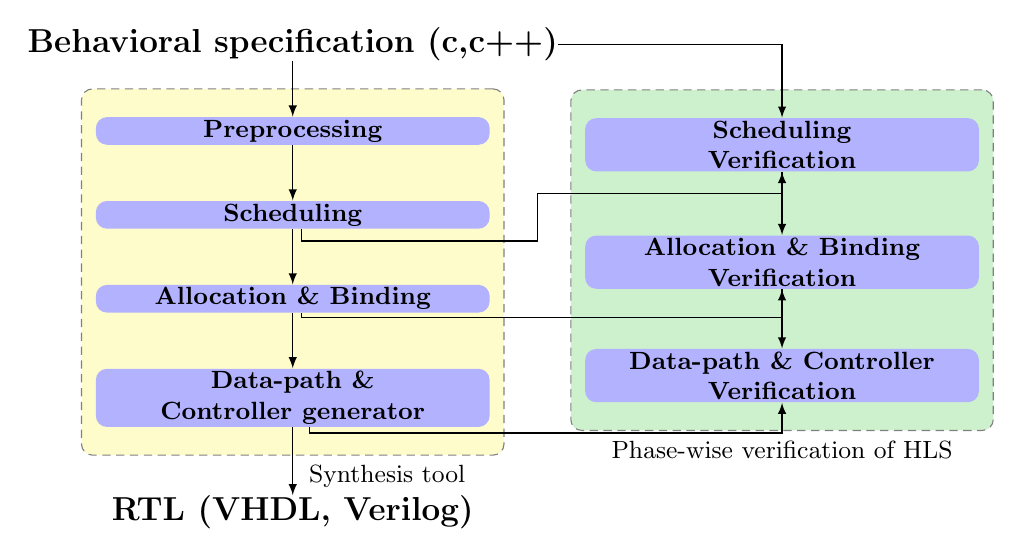
\begin{tikzpicture}
\tikzset{
mybox/.style = {fill=blue!30,
    rectangle, rounded corners, inner sep=0pt, inner ysep=1pt, text width=5cm, minimum height=0.3cm, align=center,node distance={0.7cm},font=\bfseries\small},
  back group/.style={fill=yellow!20,rounded corners, draw=black!50, densely dashed, inner xsep=5pt, inner ysep=10pt}
}
\node[inner sep=0pt](0) {\bfseries\large Behavioral specification (c,c++)};
\node[mybox,below=of 0] (1) {Preprocessing};
\node[mybox,below=of 1] (2) {Scheduling};
\node[mybox,below=of 2] (3) {Allocation \& Binding};
\node[mybox,below=of 3] (4) {Data-path \&\\ Controller generator};
\node[below=of 4, inner sep=0pt,node distance =0pt,yshift=4pt] (5) {\bfseries\large RTL (VHDL, Verilog)};
\node[temporal=<2-3>{invisible}{fvisible}{fvisible},mybox,right=of 1, xshift=0.5cm,yshift=-5pt] (6) {Scheduling\\ Verification};
\node[temporal=<2>{invisible}{fvisible}{semivisible},mybox,below=of 6,yshift=-0.1cm] (7) {Allocation \& Binding\\ Verification};
\node[temporal=<2>{invisible}{fvisible}{semivisible},mybox,below=of 7,yshift=-0.05cm] (8) {Data-path \& Controller\\ Verification};
\draw[->,>=latex] (0)--(1);
\draw[->,>=latex] (1)--(2);
\draw[->,>=latex] (2)--(3);
\draw[->,>=latex] (3)--(4);
\draw[->,>=latex] (4)--(5);
\draw[temporal=<2-3>{invisible}{fvisible}{semivisible},->,>=latex] (2.300)--++(0,-0.15)--++(3,0)--++(0,.6)-|coordinate[pos=1](b6)(6);
\draw[temporal=<2-3>{invisible}{fvisible}{semivisible},->,>=latex] (0.0)-|(6);
\draw[temporal=<2>{invisible}{fvisible}{semivisible},->,>=latex] (b6)--++(0,-0.15)-|(7);
\draw[temporal=<2>{invisible}{fvisible}{semivisible},->,>=latex] (3.300)--++(0,-0.05)-|coordinate[pos=1] (b7)(7);
\draw[temporal=<2>{invisible}{fvisible}{semivisible},->,>=latex] (b7)--++(0,-0.05)-|(8);
\draw[temporal=<2>{invisible}{fvisible}{semivisible},->,>=latex] (4.300)--++(0,-0.07)-| (8);

\begin{scope}[on background layer]
  \node[back group] (bk1)  [fit=(1) (2) (3) (4)] {};
  \end{scope}
\begin{scope}[on background layer]
  \node[temporal=<2-3>{invisible}{fvisible}{semivisible},back group,fill=green!20] (bk2)  [fit=(6) (7) (8)] {};
  \end{scope}
\node[temporal=<2-3>{invisible}{fvisible}{semivisible},below=of bk2,yshift=1cm] {\small Phase-wise verification of HLS};
\node[below=of bk1,xshift=1.2cm,yshift=1cm] {\small Synthesis tool};
\end{tikzpicture}
\end{frame}

\begin{frame}[t,fragile]
\frametitle<1-2>{Verification of HLS}
\frametitle<3-4>{Verification of HLS:Correct by Construction}
\frametitle<5-6>{Verification of HLS:Translation Validation}
\frametitle<7->{Motivation}
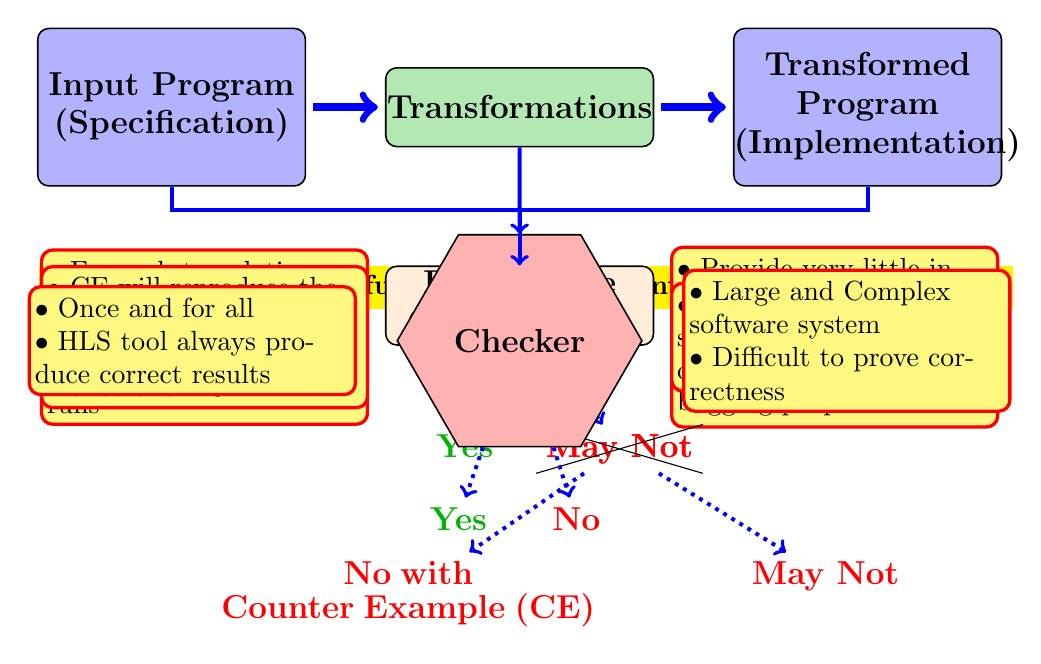
\begin{tikzpicture}
\tikzset{
mybox/.style = {draw=red, fill=yellow!50, very thick,
    rectangle, rounded corners, inner sep=2pt, inner ysep=4pt},
fstyle/.style={font=\bfseries\large,align=center,line width=0.2mm},
rect/.style={font=\bfseries\large,inner sep=0pt,rectangle,rounded corners,draw,minimum width=2cm, minimum height=2cm, text width=3.4cm, align=center,line width=0.2mm}
}
\node[temporal=<3-4>{fvisible}{semivisible}{fvisible},rect,fill=blue!30] (0) {Input Program (Specification)};
\node[temporal=<5->{fvisible}{semivisible}{fvisible},rect,right=1cm of 0,minimum height=1cm,fill=green!30] (1) {Transformations};
\node[temporal=<3-4>{fvisible}{semivisible}{fvisible},rect,right=1cm of 1,fill=blue!30] (2) {Transformed Program\\(Implementation)};

\node[temporal=<2>{invisible}{fvisible}{invisible},font=\bfseries,below= of 0,xshift=4.5cm,text width=\textwidth,align=center,fill=yellow] (3){Is the Specification ``functionally equivalent'' to Implementation?};


\node[temporal=<5->{invisible}{fvisible}{invisible},below=of 1,yshift=-0.5cm,rect,minimum height=1cm,fill=orange!15](5){Equivalence Checker (EC)};
\node[temporal=<5-6>{invisible}{fvisible}{invisible},left=of 5,text width=4cm,mybox,xshift=0.8cm,yshift=-0.4cm] (11) {$\bullet$ For each translation\\ $\bullet$ Does guarantee that any errors in translation will be caught when tool runs };
\node[temporal=<6>{invisible}{fvisible}{invisible},right=of 5,text width=4cm,mybox,xshift=-0.8cm,yshift=-0.4cm,] (12) {$\bullet$ Provide very little information in the case of nonequivalence\\ $\bullet$ Not sufficient for debugging purpose};
\node[temporal=<5->{invisible}{fvisible}{invisible},below left=of 5,xshift=2.5cm] (13) {\bfseries\large\color{green}Yes};
\node[temporal=<5-6>{invisible}{fvisible}{invisible},below right=of 5, xshift=-2.5cm] (14) {\bfseries\large\color{red}May Not};
\draw[draw=blue,temporal=<5->{invisible}{fvisible}{invisible},->,dotted] [line width=0.05cm](5) -- (13);
\draw[draw=blue,temporal=<5->{invisible}{fvisible}{invisible},->,dotted] [line width=0.05cm](5) -- (14);
\node[cross out,draw=black,temporal=<7->{invisible}{fvisible}{invisible},below right=of 5, xshift=-2.5cm] (15) {\bfseries\large\color{red}May Not};
\node[temporal=<7->{invisible}{fvisible}{invisible},below right=of 14, xshift=-.5cm] (16) {\bfseries\large\color{red}May Not};
\node[temporal=<7->{invisible}{fvisible}{invisible},below left=of 14, xshift=2cm,text width=5cm,align=center] (17) {\bfseries\large\color{red}No with\\Counter Example (CE)};
\draw[draw=blue,temporal=<7->{invisible}{fvisible}{invisible},->,dotted] [line width=0.05cm](15) -- (16);
\draw[draw=blue,temporal=<7->{invisible}{fvisible}{invisible},->,dotted] [line width=0.05cm](15) -- (17);
\node[temporal=<7->{invisible}{fvisible}{invisible},left=of 5,text width=4cm,mybox,xshift=0.8cm,yshift=-0.4cm] (18) {$\bullet$ CE will reproduce the non-equivalence\\$\bullet$ Improve the performance of a EC};
\node[temporal=<7->{invisible}{fvisible}{invisible},right=of 5,text width=4cm,mybox,xshift=-0.8cm,yshift=-0.4cm,] (19) {$\bullet$ CE helps to identify some false negative cases of a EC};

\node[temporal=<3-4>{invisible}{fvisible}{invisible},below=of 1,yshift=-0.1cm, regular polygon,regular polygon sides=6,draw,fstyle,fill=red!30](4){Checker};
\node[temporal=<3-4>{invisible}{fvisible}{invisible},left=of 4,text width=4cm,mybox,xshift=0.5cm] (7) {$\bullet$ Once and for all\\ $\bullet$ HLS tool always produce correct results};
\node[temporal=<4>{invisible}{fvisible}{invisible},mybox,right=of 4,xshift=-0.5cm,text width=4cm] (8) {$\bullet$ Large and Complex software system\\ $\bullet$ Difficult to prove correctness};
\node[temporal=<3-4>{invisible}{fvisible}{invisible},below left=of 4,xshift=1.7cm] (9) {\bfseries\large\color{green}Yes};
\node[temporal=<3-4>{invisible}{fvisible}{invisible},below right=of 4, xshift=-1.7cm] (10) {\bfseries\large\color{red}No};
\draw[draw=blue,temporal=<3-4>{invisible}{fvisible}{invisible},->,dotted] [line width=0.05cm](4) -- (9);
\draw[draw=blue,temporal=<3-4>{invisible}{fvisible}{invisible},->,dotted] [line width=0.05cm](4) -- (10);


\draw[draw=blue,temporal=<3-4>{fvisible}{semivisible}{fvisible},->][line width=0.1cm] ($(0) + (1.8,0)$) -- ($(1)+(-1.8,0)$);
\draw[draw=blue,temporal=<3-4>{fvisible}{semivisible}{fvisible},->][line width=0.1cm] ($(1) + (1.8,0)$) -- ($(2)+(-1.8,0)$);
\draw [draw=blue,temporal=<5->{invisible}{fvisible}{invisible},line width=0.05cm](0.270)-- ++(0,-0.3) -|coordinate[pos=0.25] (b2) (2);
\draw[draw=blue,->,temporal=<3-4>{invisible}{fvisible}{invisible},line width=0.05cm](1) -- (4);
\draw[draw=blue,temporal=<5->{invisible}{fvisible}{invisible},->] [line width=0.05cm](b2) -- (5);
\end{tikzpicture}
\end{frame}

\section{Path-based Equivalence Checker (PBEC)}
\begin{frame}{Path-based Equivalence Checkers (PBEC)--Related Works}
\begin{itemize}
\item C.~Karfa et al, ``\textit{An equivalence-checking method
    for scheduling verification in high-level synthesis},''IEEE TCAD, (2008).
\item Lee et al, ``\textit{Equivalence checking of scheduling with speculative code transformations in high-level 
    synthesis}'', ASP-DAC (2011).
\item K.~Banerjee et al, ``\textit{Verification of code
      motion techniques using value propagation}'', IEEE TCAD, (2014). {\color{blue}[VP Method]}
\item J. Hu et al ``Equivalence checking between SLM and RTL
using machine learning techniques," ISQED (2016).
\item R.~Chouksey et al, ``\textit{Translation validation of code motion
transformations involving loops}'', IEEE TCAD, (2018). {\color{blue}[EVP Method]}
\end{itemize}
\end{frame}
\begin{frame}{PBEC}
\begin{itemize}
\item Behaviors are represented by {\color{blue} Finite State Machine with Data (FSMD)}. 
\item Decompose each FSMD using {\color{blue} cutpoints}.
\item {\color{blue}Path}: Finite sequence of states from a cutpoint to another cutpoint.
\item {\color{blue}Equivalence of FSMDs} is established by showing path level equivalence between two FSMDs.
\end{itemize}
\end{frame}

\begin{frame}[fragile]{Representing a program using FSMD}
  \hspace*{0.5cm}
  \noindent\begin{minipage}[\textheight]{0.3\textwidth}
  \centering
  \begin{lstlisting}[language=C,
  ,numbers = none, escapechar = !,
  basicstyle = \ttfamily\bfseries, linewidth = .6\linewidth, basicstyle=\small] 
!\tikz[remember picture] \node [] (a1){};!if(n!$\geq$!0){
  x=0,y=0;!\tikz[remember picture] \node [] (a2){};!
!\tikz[remember picture] \node [] (b1){};!for(i=0;i!$\leq$!n;i++){
  x=5;
  y=y+i;}!\tikz[remember picture] \node [] (b2){};!
!\tikz[remember picture] \node [] (c1){};!out=x+y;}!\tikz[remember picture] \node [] (c2){};!
!\tikz[remember picture] \node [] (d1){};!else
out=-1;!\tikz[remember picture] \node [] (d2){};!
  \end{lstlisting}
  \end{minipage}
  \hspace*{2cm}
  \noindent\begin{minipage}[\textheight]{0.46\textwidth}
  \linespread{1.5}
  \scalebox{0.8}{
  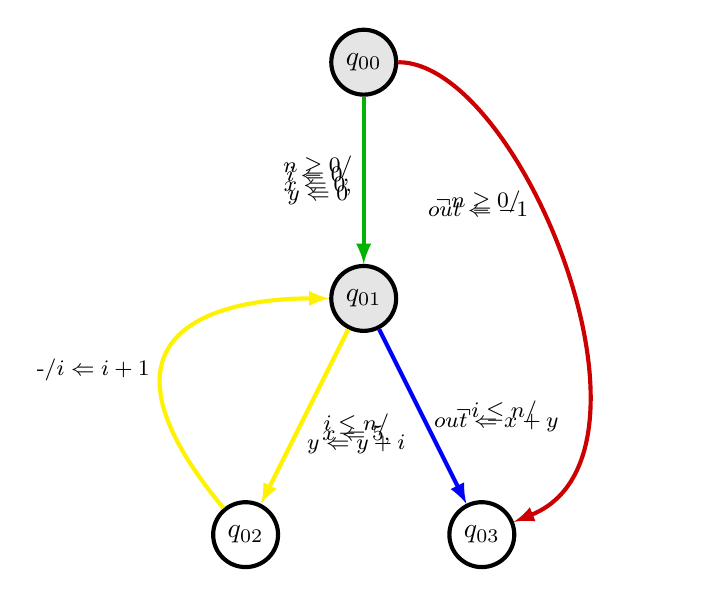
\begin{tikzpicture}[line width=1.5pt,place/.style={circle,draw,minimum size=8mm}]
    \node[fill=gray!20] (1) at (0,1)   [place] {$q_{00}$};
    \node[fill=gray!20] (2) at (0,-2)   [place] {$q_{01}$};
    \node (3) at (-1.5,-5)   [place] {$q_{02}$};
    \node (5) at (1.5,-5)   [place] {$q_{03}$};
    
    \draw [>=latex,->,draw=green](1) to [align=center] node[pos=0.5,left] {\footnotesize $n\geq 0/$\\[-0.3cm] \footnotesize $i\Leftarrow 0,$\\[-0.3cm]\footnotesize $x\Leftarrow 0,$\\[-0.3cm]\footnotesize $y\Leftarrow 0$}(2);
    
    \draw [>=latex,->,draw=yellow](2)  [align=center] to  node[pos=0.6,right] {\footnotesize$i\leq n/$\\[-0.3cm]\footnotesize $x\Leftarrow 5,$\\[-0.3cm]\footnotesize $y\Leftarrow y+i$}(3);
    
    \draw [>=latex,->,draw=yellow](3) [align=center] .. controls (-4,-2) and (-1,-2) ..  
    node[pos=0.3,left] {\footnotesize -/\footnotesize$i\Leftarrow i+1$}(2);
    
    \draw [>=latex,->,draw=blue](2)  [align=center] --node[pos=0.5,right]{\footnotesize$\neg i\leq n/$\\[-0.3cm]\footnotesize$out\Leftarrow x+y$}(5);
    
    \draw [>=latex,->,draw=boston](1)  [align=center] .. controls (2,1) and (4,-4) ..  
    node[pos=0.4,left] {\footnotesize $\neg n\geq 0$/\\[-0.3cm]\footnotesize$out\Leftarrow -1$} (5);
    
    %\draw [>=latex,->](5) .. controls (6,-4)  and (2,2) .. node[pos=0.6,right] {\footnotesize $-/-$} (1); 
  \end{tikzpicture}
  }
  \end{minipage}
  \begin{tikzpicture}[remember picture, overlay]
  \draw[->,thick,draw=green] ($(a1)+(-0.2,0.3)$) rectangle ($(a2)+(0.2,-0.2)$);
  \draw[->,thick,draw=yellow] ($(b1)+(-0.2,0.16)$) rectangle ($(b2)+(2.3,-0.2)$);
  \draw[->,draw=blue,thick] ($(c1)+(-0.2,0.16)$) rectangle ($(c2)+(0.2,-0.2)$);
  \draw[->,draw=boston,thick] ($(d1)+(-0.2,0.16)$) rectangle ($(d2)+(0.2,-0.2)$);
  \end{tikzpicture}
\end{frame}



\section{Overall Approach}
\begin{frame}{Overall Approach}
In the case of nonequivalence reported by PBEC
\begin{enumerate}
\item Counter Trace ({\color{blue}$\mathit{cTrace}$}) {\color{blue}generation}. 
\item {\color{blue}Modeling} the $\mathit{cTrace}$ to generate counter example using {\color{blue}CBMC}.
\item {\color{blue}Incorporate} the results with PBEC.
\end{enumerate}
\end{frame}
%\subsection{$\mathit{cTrace}$ Generation}
\tikzstyle{highlightGreen}=[line width=1.5pt,draw=green]
\tikzstyle{highlightYellow}=[line width=1.5pt,draw=yellow]
\tikzstyle{highlightRed}=[line width=1.5pt,draw=red]

\begin{frame}{$\mathit{cTrace}$ Generation in the EVP Method}
\begin{minipage}[\textheight]{0.45\textwidth}
	\centering
		\begin{figure}[!h]
			\linespread{1.5}
			\scalebox{0.75}{
				\begin{tikzpicture}[line width=1.5pt,place/.style={circle,draw}]
					\node (10) at (0,2) {$M_0$};
				%%%%%%%%%%%%%%%%%%%%%%%%%%%M0%%%%%%%%%%%%%%%%%%%%%%
					\node[fill=gray!20] (1) at (0,1)   [place] {$q_{00}$};
					\node[fill=gray!20] (2) at (0,-2)   [place] {$q_{01}$};
					\node (3) at (-1.5,-5)   [place] {$q_{02}$};
					\node (5) at (1.5,-5)   [place] {$q_{03}$};
					
					\draw [onslide=<3->{highlightGreen},>=latex,->](1) to [align=center] node[pos=0.5,left] {\footnotesize $n\geq 0/$\\[-0.3cm] \footnotesize $i\Leftarrow 0,$\\[-0.3cm]\footnotesize $x\Leftarrow 0,$\\[-0.3cm]\footnotesize $y\Leftarrow 0$} 
					node[onslide=<1-2>{invisible},onslide=<3->,pos=0.4,right]{$P_{01}$} (2);
					
					\draw [onslide=<4->{highlightYellow},>=latex,->](2)  [align=center] to  node[pos=0.6,right] {\footnotesize$i\leq n/$\\[-0.3cm]\footnotesize $\boxed{\mathbf{x\Leftarrow 5}},$\\[-0.3cm]\footnotesize $y\Leftarrow y+5$}(3);
					
					\draw [onslide=<4->{highlightYellow},>=latex,->](3) [align=center] .. controls (-3,-2) and (-0.8,-2) ..  node[pos=0.3,left] {\rotatebox[origin=c]{90}{\footnotesize -/\footnotesize$i\Leftarrow i+1$}} 	node[onslide=<1-3>{invisible},onslide=<4->,pos=0.3,right,xshift=0.3cm]{$P_{02}$}(2);
					
					\draw [onslide=<5->{highlightRed},>=latex,->](2)  [align=center] --node[pos=0.5,right]{\footnotesize$\neg i\leq n/$\\[-0.3cm]\footnotesize{\boxed{\mathbf{out\Leftarrow x+y}}}}
					node[onslide=<1-4>{invisible},onslide=<5->,pos=0.8,right]{$P_{03}$}(5);
					
					\draw [onslide=<2->{highlightGreen},>=latex,->](1)  [align=center] .. controls (2,1) and (5,-4) ..  
					node[pos=0.4,left] {\footnotesize $\neg n\geq 0$/\\[-0.3cm]\footnotesize$out\Leftarrow -1$} node[pos=0.4,right,onslide=<1>{invisible},onslide=<2->]{$P_{00}$} (5);
									
				\end{tikzpicture}
				}
				\end{figure}
				\end{minipage}
\begin{minipage}[\textheight]{0.45\textwidth}
	\centering
		\begin{figure}[!h]
			\linespread{1.5}
			\scalebox{0.75}{
				\begin{tikzpicture}[line width=1.5pt,place/.style={circle,draw}]
					\node (10) at (0,2) {$M_1$};
				%%%%%%%%%%%%%%%%%%%%%%%%%%%M0%%%%%%%%%%%%%%%%%%%%%%
					\node[fill=gray!20] (1) at (0,1)   [place] {$q_{10}$};
					\node[fill=gray!20] (2) at (0,-2)   [place] {$q_{11}$};
					\node (3) at (-1.5,-5)   [place] {$q_{12}$};
					\node (5) at (1.5,-5)   [place] {$q_{13}$};
					
					\draw [onslide=<3->{highlightGreen},>=latex,->](1) to [align=center] node[pos=0.5,left] {\footnotesize $n\geq 0/$\\[-0.3cm] \footnotesize $i\Leftarrow 0,$\\[-0.3cm]\footnotesize $x\Leftarrow 0,$\\[-0.3cm]\footnotesize $y\Leftarrow 0$}
					node[onslide=<1-2>{invisible},onslide=<3->,pos=0.4,right]{$P_{11}$}
					(2);
					
					\draw[onslide=<4->{highlightYellow},>=latex,->](2)  [align=center] to  node[pos=0.6,right] {\footnotesize$i\leq n/$\\[-0.3cm]\footnotesize $y\Leftarrow y+5$}(3);
					
					\draw [onslide=<4->{highlightYellow},>=latex,->](3) [align=center] .. controls (-3,-2) and (-0.8,-2) ..  
					node[pos=0.3,left] {\rotatebox[origin=c]{90}{\footnotesize -/\footnotesize$i\Leftarrow i+1$}}
					node[onslide=<1-3>{invisible},onslide=<2->,pos=0.3,right,xshift=0.3cm]{$P_{12}$}(2);
					
					\draw [onslide=<5->{highlightRed},>=latex,->](2)  [align=center] --node[pos=0.3,right,]{\footnotesize$\neg i\leq n/$\\[-0.3cm]\footnotesize $\boxed{\mathbf{x\Leftarrow 5}},$\\[-0.2cm]\footnotesize
					${\boxed{\mathbf{out\Leftarrow x+y+1}}}$}
					node[onslide=<1-4>{invisible},onslide=<2->,pos=0.8,right]{$P_{13}$}
					(5);
					
					\draw [onslide=<2->{highlightGreen},>=latex,->](1)  [align=center] .. controls (2,1) and (5,-4) ..  
					node[pos=0.4,left] {\footnotesize $\neg n\geq 0$/\\[-0.3cm]\footnotesize$out\Leftarrow -1$} node[onslide=<1>{invisible},onslide=<2->,pos=0.4,right]{$P_{10}$} (5);
					
				\end{tikzpicture}
				}
				\end{figure}
		\end{minipage}
		\begin{overlayarea}{\textwidth}{5cm} 
		\vspace{0.05cm}
		\scalebox{0.7}{
		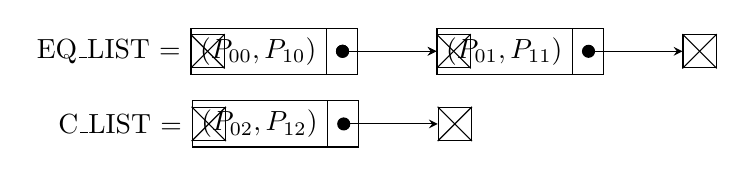
\begin{tikzpicture}[list/.style={rectangle split, rectangle split parts=2,
		    draw, rectangle split horizontal}, >=stealth]
		  \node (A) {EQ\_LIST = };
		 	\node[below=of A,yshift=0.6cm,xshift=0.145cm] (B) {C\_LIST = };
		  
		  \node[onslide=<2->{invisible},right=of A,xshift=-1cm,draw,inner sep=6pt] (A1) {};
		  \node[onslide=<4->{invisible},right=of B,xshift=-1cm,draw,inner sep=6pt] (B1) {};
		  
		  \node[onslide=<1>{invisible},list,right=of A,xshift=-1cm,] (A2) {$(P_{00},P_{10})$};
		  \node[onslide=<1>{invisible},onslide=<3->{invisible},right=of A2,draw,inner sep=6pt] (A21) {};
			
			\node[onslide=<1-2>{invisible},list,right=of A2] (A3) {$(P_{01},P_{11})$};
			\node[onslide=<1-2>{invisible},right=of A3,draw,inner sep=6pt] (A31) {};

			\node[onslide=<1-3>{invisible},list,right=of B,xshift=-1cm,] (B2) {$(P_{02},P_{12})$};
			\node[onslide=<1-3>{invisible},right=of B2,draw,inner sep=6pt] (B21) {};
		  
		  \draw[onslide=<2->{invisible}] (A1.north east) -- (A1.south west);
		  \draw[onslide=<2->{invisible}] (A1.north west) -- (A1.south east);
			
			\draw[onslide=<4->{invisible}] (B1.north east) -- (B1.south west);
		  \draw[onslide=<4->{invisible}] (B1.north west) -- (B1.south east);
		  
		  \draw[onslide=<1>{invisible},onslide=<3->{invisible}] (A21.north east) -- (A21.south west);
		  \draw[onslide=<1>{invisible},onslide=<3->{invisible}] (A21.north west) -- (A21.south east);
		  
		  \draw[onslide=<1-2>{invisible}] (A31.north east) -- (A31.south west);
		  \draw[onslide=<1-2>{invisible}] (A31.north west) -- (A31.south east);
		
			\draw[onslide=<1-3>{invisible}] (B21.north east) -- (B21.south west);
			\draw[onslide=<1-3>{invisible}] (B21.north west) -- (B21.south east);
		  			
		  
		  \draw[onslide=<1>{invisible},onslide=<3->{invisible},*->] let \p1 = (A2.two), \p2 = (A2.center) in (\x1,\y2) -- (A21);
		  \draw[onslide=<1-2>{invisible},*->] let \p1 = (A2.two), \p2 = (A2.center) in (\x1,\y2) -- (A3);
		  \draw[onslide=<1-2>{invisible},*->] let \p1 = (A3.two), \p2 = (A3.center) in (\x1,\y2) -- (A31);
		  \draw[onslide=<1-3>{invisible},*->] let \p1 = (B2.two), \p2 = (B2.center) in (\x1,\y2) -- (B21);
		\end{tikzpicture}
		}																		
		\end{overlayarea}
		\end{frame}
		%%%%%%%%%%%%%%%%%%%%%%%%%%%%%%%%%%%%%%%%%%%%%%%%%%%%%%%%%%%%%%%%%%%%%%%%%%%%
		\begin{frame}[t]{$\mathit{cTrace}$ Generation in EVP Method}
		\tikzstyle{every picture}+=[remember picture]
		In case of nonequivalence
		\begin{itemize}
		\item\visible<2-5> {Can not find equivalent path (say $\alpha$)} \tikz \node[coordinate] (n1) {};
		\item\visible<3-5> {C\_LIST} \tikz \node[coordinate] (n2) {};
		\item\visible<4-5> {Paths from EQ\_LIST} \tikz \node[coordinate] (n3) {}; 
		\item\visible<5>{$\mathit{cTrace}$ of $M_0$ and $M_1$}
		\end{itemize}
		\vspace{0.6cm}
		\begin{tikzpicture}[overlay]
		\node(0) {};
		\node[right=of 0] (1){$\mathit{cTrace}$ of $M_0=\langle$};
		\node[onslide=<1-3>{invisible},fill=green!20,right=of 1,xshift=-1cm] (2) {$P_{00},P_{01},\cdots,P_{0i},$}; 
		\node[onslide=<1-2>{invisible},fill=red!20,right=of 2,xshift=-1cm] (3) {$P_{0j},P_{0j+1},\cdots,P_{0k},$}; 
		\node[onslide=<1>{invisible},fill=blue!20,right=of 3,xshift=-1cm] (4) {$\alpha$};
		\node[right=of 4,xshift=-1cm] (5) {$\rangle$};
		\node[below =of 1,onslide=<1-4>{invisible}] (6) {$\mathit{cTrace}$ of $M_1=\langle$};
		\node[onslide=<1-4>{invisible},fill=green!20,right=of 6,xshift=-1cm] (7) {$P_{10},P_{11},\cdots,P_{1i},$}; 
		\node[onslide=<1-4>{invisible},fill=red!20,right=of 7,xshift=-1cm] (8) {$P_{1j},P_{1j+1},\cdots,P_{1k},$}; 
		\node[onslide=<1-4>{invisible},fill=blue!20,right=of 8,xshift=-1cm] (9) {$\beta$};
		\node[onslide=<1-4>{invisible},right=of 9,xshift=-1cm] (10) {$\rangle$};
		\path[->,onslide=<1>{invisible},line width=0.03cm] (n1) edge [bend left] (4);
		\path[->,onslide=<1-2>{invisible},line width=0.03cm] (n2) edge [bend left] (3);
		\path[->,onslide=<1-3>{invisible},line width=0.03cm] (n3) edge [bend left] (2);
		\end{tikzpicture}
		\end{frame}
		%%%%%%%%%%%%%%%%%%%%%%%%%%%%%%%%%%%%%%%%%%%%%%%%%%%%%%%%%%%%%%%%%%%%%%%%%%%
		\begin{frame}{$\mathit{cTrace}$ Generation in EVP Method}
		\begin{minipage}[\textheight]{0.45\textwidth}
			\centering
				\begin{figure}[!h]
					\linespread{1.5}
					\scalebox{0.75}{
						\begin{tikzpicture}[line width=1.5pt,place/.style={circle,draw}]
							\node (10) at (0,2) {$\mathit{cTrace}$ of $M_0$};
						%%%%%%%%%%%%%%%%%%%%%%%%%%%M0%%%%%%%%%%%%%%%%%%%%%%
							\node[fill=gray!20] (1) at (0,1)   [place] {$q_{00}$};
							\node[fill=gray!20] (2) at (0,-2)   [place] {$q_{01}$};
							\node (3) at (-1.5,-5)   [place] {$q_{02}$};
							\node (5) at (1.5,-5)   [place] {$q_{03}$};
							
							\draw [onslide=<1->{highlightGreen},>=latex,->](1) to [align=center] node[pos=0.5,left] {\footnotesize $n\geq 0/$\\[-0.3cm] \footnotesize $i\Leftarrow 0,$\\[-0.3cm]\footnotesize $x\Leftarrow 0,$\\[-0.3cm]\footnotesize $y\Leftarrow 0$} 
							node[pos=0.4,right]{$P_{01}$} (2);
							
							\draw [onslide=<1->{highlightYellow},>=latex,->](2)  [align=center] to  node[pos=0.6,right] {\footnotesize$i\leq n/$\\[-0.3cm]\footnotesize $\boxed{\mathbf{x\Leftarrow 5}},$\\[-0.3cm]\footnotesize $y\Leftarrow y+5$}(3);
							
							\draw [onslide=<1->{highlightYellow},>=latex,->](3) [align=center] .. controls (-3,-2) and (-0.8,-2) ..  node[pos=0.3,left] {\rotatebox[origin=c]{90}{\footnotesize -/\footnotesize$i\Leftarrow i+1$}} 	node[pos=0.3,right,xshift=0.3cm]{$P_{02}$}(2);
							
							\draw [onslide=<1->{highlightRed},>=latex,->](2)  [align=center] --node[pos=0.5,right]{\footnotesize$\neg i\leq n/$\\[-0.3cm]\footnotesize$\boxed{\mathbf{out\Leftarrow x+y}}$}
							node[pos=0.8,right]{$P_{03}$}(5);				
						\end{tikzpicture}
						}
						\end{figure}
						\end{minipage}
		\begin{minipage}[\textheight]{0.45\textwidth}
			\centering
				\begin{figure}[!h]
					\linespread{1.5}
					\scalebox{0.75}{
						\begin{tikzpicture}[line width=1.5pt,place/.style={circle,draw}]
							\node (10) at (0,2) {$\mathit{cTrace}$ of $M_1$};
						%%%%%%%%%%%%%%%%%%%%%%%%%%%M0%%%%%%%%%%%%%%%%%%%%%%
							\node[fill=gray!20] (1) at (0,1)   [place] {$q_{10}$};
							\node[fill=gray!20] (2) at (0,-2)   [place] {$q_{11}$};
							\node (3) at (-1.5,-5)   [place] {$q_{12}$};
							\node (5) at (1.5,-5)   [place] {$q_{13}$};
							
							\draw [onslide=<1->{highlightGreen},>=latex,->](1) to [align=center] node[pos=0.5,left] {\footnotesize $n\geq 0/$\\[-0.3cm] \footnotesize $i\Leftarrow 0,$\\[-0.3cm]\footnotesize $x\Leftarrow 0,$\\[-0.3cm]\footnotesize $y\Leftarrow 0$}
							node[pos=0.4,right]{$P_{11}$}
							(2);
							
							\draw[onslide=<1->{highlightYellow},>=latex,->](2)  [align=center] to  node[pos=0.6,right] {\footnotesize$i\leq n/$\\[-0.3cm]\footnotesize $y\Leftarrow y+5$}(3);
							
							\draw [onslide=<1->{highlightYellow},>=latex,->](3) [align=center] .. controls (-3,-2) and (-0.8,-2) ..  
							node[pos=0.3,left] {\rotatebox[origin=c]{90}{\footnotesize -/\footnotesize$i\Leftarrow i+1$}}
							node[pos=0.3,right,xshift=0.3cm]{$P_{12}$}(2);
							
							\draw [onslide=<1->{highlightRed},>=latex,->](2)  [align=center] --node[pos=0.3,right,]{\footnotesize$\neg i\leq n/$\\[-0.3cm]\footnotesize $\boxed{\mathbf{x\Leftarrow 5}},$\\[-0.2cm]\footnotesize$\boxed{\mathbf{out\Leftarrow x+y+1}}$}
							node[pos=0.8,right]{$P_{13}$}
							(5);
						\end{tikzpicture}
						}
						\end{figure}
				\end{minipage}
				
				\begin{overlayarea}{\textwidth}{5cm} 
				\vspace{0.2cm}
				\scalebox{0.6}{
				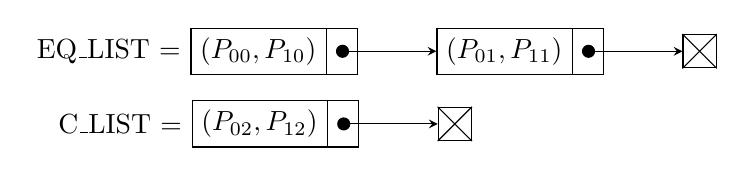
\begin{tikzpicture}[list/.style={rectangle split, rectangle split parts=2,
				    draw, rectangle split horizontal}, >=stealth]
				  
				  \node (A) {EQ\_LIST = };
				 	\node[list,right=of A,xshift=-1cm,] (A2) {$(P_{00},P_{10})$};
				  \node[list,right=of A2] (A3) {$(P_{01},P_{11})$};
					\node[right=of A3,draw,inner sep=6pt] (A31) {};
		
					\node[below=of A,yshift=0.6cm,xshift=0.145cm] (B) {C\_LIST = };			  
					\node[list,right=of B,xshift=-1cm,] (B2) {$(P_{02},P_{12})$};
					\node[right=of B2,draw,inner sep=6pt] (B21) {};
				  				  
				 
				  \draw(A31.north east) -- (A31.south west);
				  \draw(A31.north west) -- (A31.south east);
				
					\draw(B21.north east) -- (B21.south west);
					\draw(B21.north west) -- (B21.south east);
				  			
				  
				  \draw[*->] let \p1 = (A2.two), \p2 = (A2.center) in (\x1,\y2) -- (A3);
				  \draw[*->] let \p1 = (A3.two), \p2 = (A3.center) in (\x1,\y2) -- (A31);
				  \draw[*->] let \p1 = (B2.two), \p2 = (B2.center) in (\x1,\y2) -- (B21);
				\end{tikzpicture}
				}																		
				\end{overlayarea}
				\end{frame}

%\subsection{Counter Example Generation}
\tikzstyle{highlightGreen}=[line width=1.5pt,draw=green]
\begin{frame}[fragile]
\begin{overlayarea}{\textwidth}{15cm} 
\begin{tikzpicture}[remember picture,line width=1.5pt,]
\tikzset{
mybox/.style = {draw=red, fill=yellow!50, very thick,
    rectangle, rounded corners, inner sep=2pt, inner ysep=4pt}
}
\node[draw=black,temporal=<2>{fvisible}{highlightGreen}{semivisible},text width=0.45\textwidth,inner sep=0pt](a)
{%
\begin{minipage}[t]{\textwidth}%
\noindent
\begin{lstlisting}[language=C,escapechar=~]
#include<assert.h>
void main()
{
  int i_s,x_s,y_s,n,out_s;
  int i_t,x_t,y_t,out_t;
  __CPROVER_assume(n>=0);
  assert(!(n>=0));
\end{lstlisting}
\end{minipage}};
\node[draw=black,temporal=<3>{fvisible}{highlightGreen}{semivisible},onslide=<2>{semivisible},below=of a,text width=0.45\textwidth,inner sep=0pt,yshift=0.8cm] (b){%
\begin{minipage}{\textwidth}%
\noindent
\begin{lstlisting} [language=C,escapechar=~,firstnumber=8]
// cTrace for M0
  if(n>=0)
  {
    i_s=0;x_s=0;y_s=0;
    __CPROVER_assume(i_s<=n);
    assert(!(i_s<=n));
    while(i_s<=n)
    {
      x_s=5;
      y_s=y_s+5;
      i_s=i_s+1;
    }
    out_s=x_s+y_s;
  }
\end{lstlisting}
\end{minipage}};
\node[draw=black,temporal=<4>{fvisible}{highlightGreen}{semivisible},onslide=<2-3>{semivisible},right=of b,text width=0.47\textwidth,inner sep=1pt,yshift=3cm] (c){%
\begin{minipage}{\textwidth}%
\noindent
\begin{lstlisting} [language=C,escapechar=~,firstnumber=22]
//cTrace for M1
  if(n>=0)
  {
    i_t=0;x_t=0;y_t=0;
    __CPROVER_assume(i_t<=n);
    assert(!(i_t<=n));
    while(i_t<=n)
    {
      y_t=y_t+5;
      i_t=i_t+1;
    }
    x_t=5;
    out_t=x_t+y_t+1;
  }
\end{lstlisting}
\end{minipage}};
\node[draw=black,temporal=<5>{fvisible}{highlightGreen}{semivisible},onslide=<2-4>{semivisible},below=of c,text width=0.47\textwidth,yshift=0.8cm,inner sep=1pt] (d) 
{%
\begin{minipage}{\textwidth}%
\noindent
\begin{lstlisting}[language=C,escapechar=~,firstnumber=36]
//Live variables
  assert(x_s = x_t);
  assert(y_s = y_t);
//Output variable
 assert(out_s = out_t);
}
\end{lstlisting}
\end{minipage}};

\node[temporal=<2>{invisible}{fvisible}{invisible},mybox,below=of c,xshift=-3cm,yshift=3cm,text width=10cm]
{\begin{minipage}{\textwidth}
\begin{itemize}
\item \_s -- Variables appearing in the cTrace of $M_0$.
\item \_t -- Variables appearing in the cTrace of $M_1$.
\item n -- common Variable.
\item $\mathtt{\_\_CPROVER\_assume}$ -- allow only those computations that satisfy a given condition.
\end{itemize}\end{minipage}};

\node[temporal=<3>{invisible}{fvisible}{invisible},mybox,inner sep=0pt,right=of b,yshift=2cm,xshift=-0.45cm]
{\begin{minipage}[t]{0.5\textwidth}
\linespread{1.5}
\begin{tikzpicture}[line width=1.5pt,place/.style={circle,draw}]
        %%%%%%%%%%%%%%%%%%%%%%%%%%%M0%%%%%%%%%%%%%%%%%%%%%%
          \node[fill=gray!20] (1) at (0,1)   [place] {$q_{00}$};
          \node[fill=gray!20] (2) at (0,-2)   [place] {$q_{01}$};
          \node (3) at (-1.5,-5)   [place] {$q_{02}$};
          \node (5) at (1.5,-5)   [place] {$q_{03}$};
          
          \draw [>=latex,->,draw=green](1) to [align=center] node[pos=0.5,left] 
          {\footnotesize $n\geq 0/$\\[-0.3cm] \footnotesize $i\Leftarrow 
          0,$\\[-0.3cm]\footnotesize $x\Leftarrow 0,$\\[-0.3cm]\footnotesize 
          $y\Leftarrow 0$} 
          node[pos=0.4,right]{$p_{01}$} (2);
          
          \draw [>=latex,->,draw=yellow](2)  [align=center] to  
          node[pos=0.6,right] {\footnotesize$i\leq n/$\\[-0.2cm]\footnotesize 
          $\boxed{\mathbf{x\Leftarrow 5}},$\\[-0.3cm]\footnotesize $y\Leftarrow 
          y+5$}(3);
          
          \draw [>=latex,->, draw=yellow](3) [align=center] .. controls (-3,-2) 
          and (-0.8,-2) ..  node[pos=0.3,left] 
          {\rotatebox[origin=c]{90}{\footnotesize -/\footnotesize$i\Leftarrow 
          i+1$}}  node[pos=0.3,right,xshift=0.3cm]{$p_{02}$}(2);
          
          \draw [>=latex,->,draw=red](2)  [align=center] 
          --node[pos=0.5,right]{\footnotesize$\neg i\leq 
          n/$\\[-0.2cm]\footnotesize{\boxed{\mathbf{out\Leftarrow x+y}}}}
          node[pos=0.8,right]{$p_{03}$}(5);       
        \end{tikzpicture}
\end{minipage}};

\node[temporal=<4>{invisible}{fvisible}{invisible},mybox,inner sep=0pt,left=of d,yshift=3cm,xshift=0.7cm]
{\begin{minipage}[t]{0.5\textwidth}
\linespread{1.5}
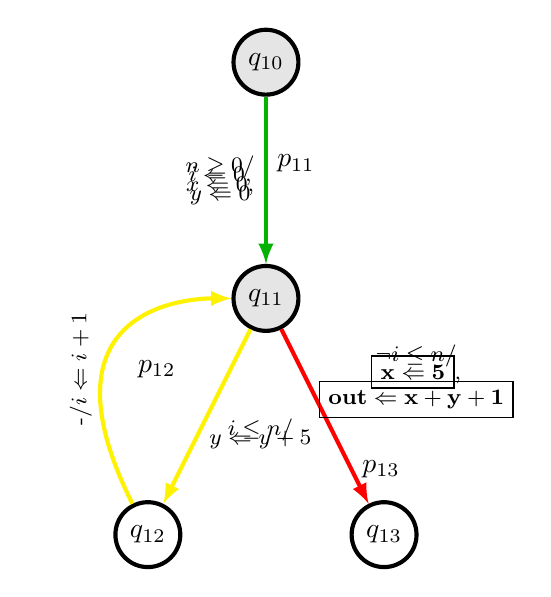
\begin{tikzpicture}[line width=1.5pt,place/.style={circle,draw}]
        %%%%%%%%%%%%%%%%%%%%%%%%%%%M0%%%%%%%%%%%%%%%%%%%%%%
          \node[fill=gray!20] (1) at (0,1)   [place] {$q_{10}$};
          \node[fill=gray!20] (2) at (0,-2)   [place] {$q_{11}$};
          \node (3) at (-1.5,-5)   [place] {$q_{12}$};
          \node (5) at (1.5,-5)   [place] {$q_{13}$};
          
          \draw [>=latex,->,draw=green](1) to [align=center] node[pos=0.5,left] 
          {\footnotesize $n\geq 0/$\\[-0.3cm] \footnotesize $i\Leftarrow 
          0,$\\[-0.3cm]\footnotesize $x\Leftarrow 0,$\\[-0.3cm]\footnotesize 
          $y\Leftarrow 0$}
          node[pos=0.4,right]{$p_{11}$}
          (2);
          
          \draw[>=latex,->,draw=yellow](2)  [align=center] to  
          node[pos=0.6,right] {\footnotesize$i\leq n/$\\[-0.3cm]\footnotesize 
          $y\Leftarrow y+5$}(3);
          
          \draw [>=latex,->,draw=yellow](3) [align=center] .. controls (-3,-2) 
          and (-0.8,-2) ..  
          node[pos=0.3,left] {\rotatebox[origin=c]{90}{\footnotesize 
          -/\footnotesize$i\Leftarrow i+1$}}
          node[pos=0.3,right,xshift=0.3cm]{$p_{12}$}(2);
          
          \draw [>=latex,->,draw=red](2)  [align=center] 
          --node[pos=0.3,right,]{\footnotesize$\neg i\leq 
          n/$\\[-0.2cm]\footnotesize $\boxed{\mathbf{x\Leftarrow 
          5}},$\\[-0.1cm]\footnotesize
          ${\boxed{\mathbf{out\Leftarrow x+y+1}}}$}
          node[pos=0.8,right]{$p_{13}$}
          (5);
        \end{tikzpicture}
\end{minipage}};
\node[temporal=<5>{invisible}{fvisible}{invisible},mybox,above=of d,xshift=-3cm,yshift=1cm,text width=10cm]
{\begin{minipage}{\textwidth}
\begin{itemize}
\item CBMC verifies the specified assertions. 
\item If any violation of an assertion is detected, a counter-example is
generated.
\item $n = 0$ the values of the variable `out' differs.
\end{itemize}\end{minipage}};

\end{tikzpicture}
\end{overlayarea}
\end{frame}

%\subsection{Incorporating the Results}
\begin{frame}{PBEC+Counter Exmaple Generator (CEG)}
\begin{figure*}[!t]
 \centering
 \scalebox{0.34}{
 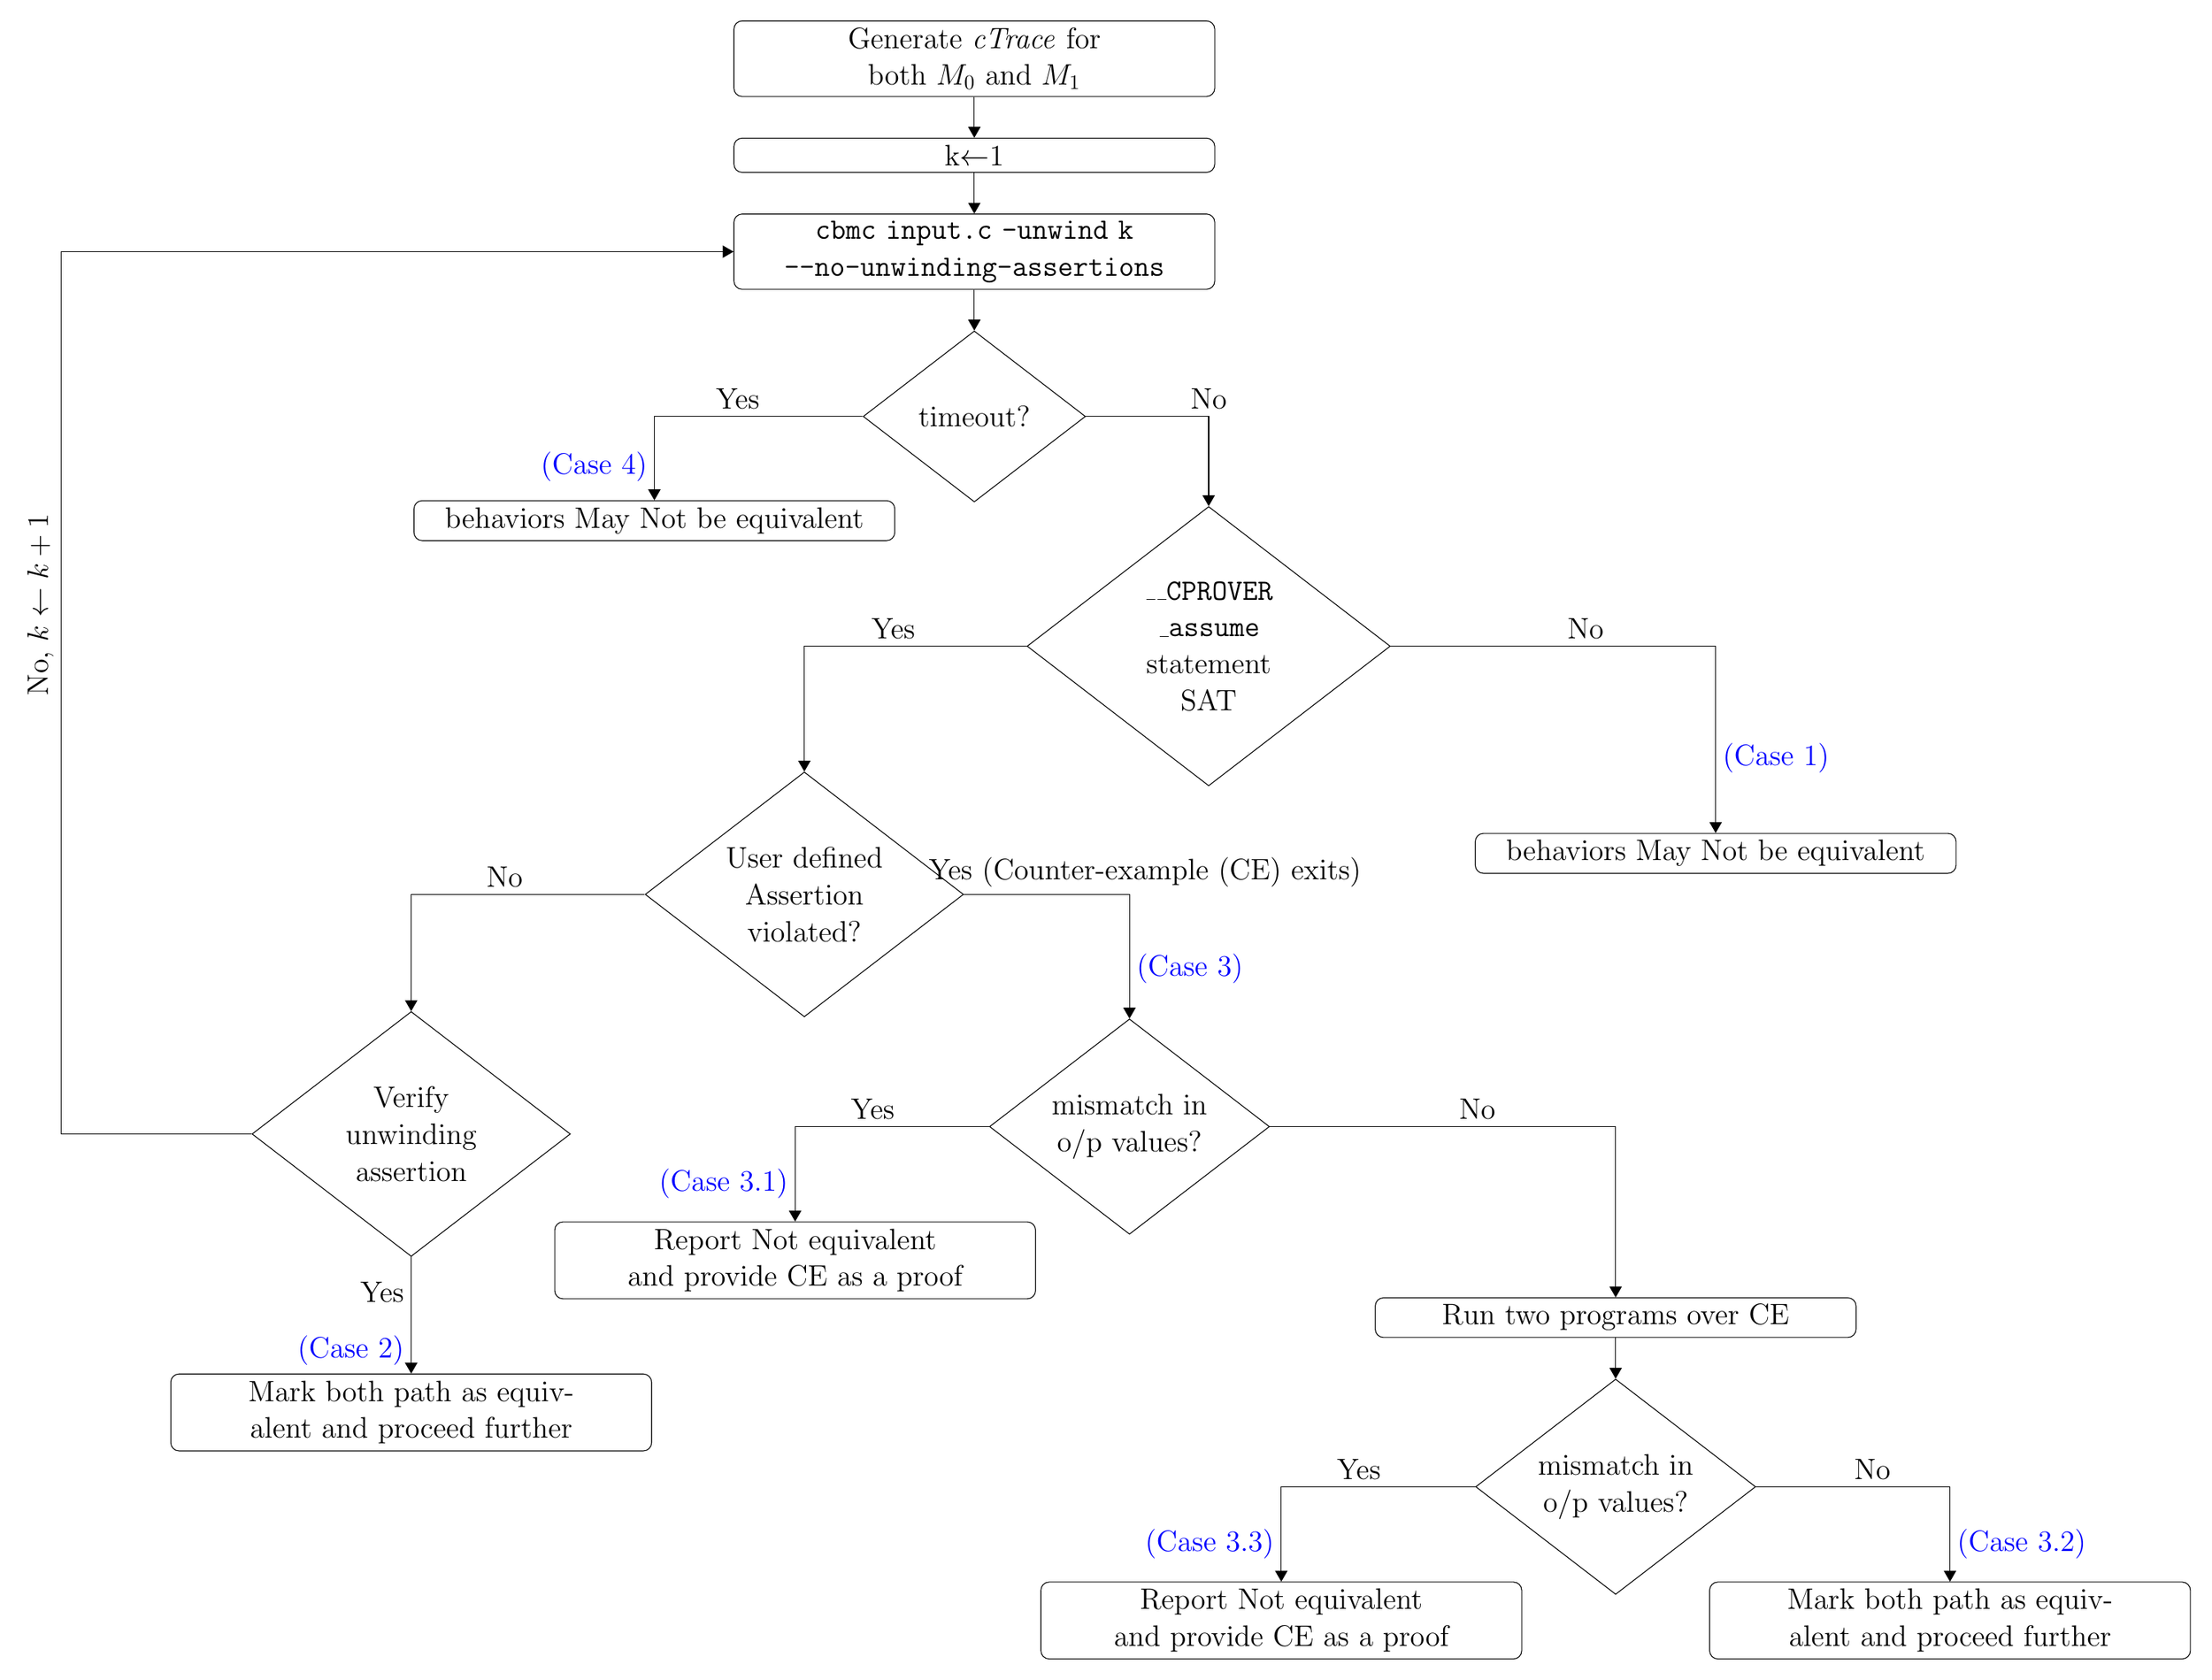
\begin{tikzpicture}[%
      >=triangle 60,              % Nice arrows; your taste may be different
      node distance=7mm and 4mm, % Global setup of box spacing
      every join/.style={norm},   % Default linetype for connecting boxes
 	   font=\Large,auto
      ]
  \tikzset{
 	 rect/.style={draw,align=center,rectangle, text width=8cm,rounded corners},	
 	 test/.style={draw, align=center,diamond, aspect=1.3, text width=8em}}
 \node [rect] (1) {Generate $\mathit{cTrace}$ for both $M_0$ and $M_1$};
 
  \node [rect,below=of 1] (12)     {k$\leftarrow$1};
 \node [rect,below=of 12] (2)     {\texttt{cbmc input.c -unwind k 
 --no-unwinding-assertions}};
 
 \node [test,below=of 2]  (t1)    {timeout?};
 
 \node [rect,below left=of t1]   (3)    {behaviors May Not be equivalent};
 
 \node [test,node distance=2cm and 1.5cm,below right=of t1]  (t2) 
 {\texttt{\_\_CPROVER\\\_assume} statement  SAT};
 
 \node [test,node distance=2cm and 4cm,below left=of t2]  (t3)    {User 
defined Assertion violated?};
 
 \node [rect,node distance=2cm and 3cm,below right=of t2]   (4)    {behaviors 
 May Not be equivalent};


\node [test,node distance=2cm and 4cm,below left=of t3]  (t21) {Verify 
 unwinding assertion};
  
 \node [rect,node distance=2cm and 5cm,below =of t21]   (6)  {Mark both path 
 as equivalent and proceed further};
 
 
 \node [test,node distance=2cm and 3cm,below right=of t3]  (t6)    {mismatch 
 in o/p values?};
 
 \node [rect,below left=of t6]  (r6)    {Report Not equivalent and provide CE 
 as a proof};
 
 \node [rect,node distance=2cm and 3cm,below right=of t6,] (5)     {Run two 
 programs over CE};
 
 \node [test,below=of 5]  (t4)    {mismatch in o/p values?};
 
 
 
 \node [rect,below right=of t4]   (7)  {Mark both path as equivalent and 
 proceed further};
 
 \node [rect,below left=of t4]  (8)    {Report Not equivalent and provide CE 
 as  a proof};
 
 
 \draw[->] (1) -- (12);
 \draw[->] (12) -- (2);
 \draw[->] (2) -- (t1);
 \draw[->]  (t1.180) -| node[pos=0.3,above]{Yes} node[pos=0.8,left]{\color{blue}{(Case~4)}} (3);
 \draw[->] (t1.0) -| node[above]{No} (t2.90);
 \draw[,->]  (t2.0) -| node[pos=0.3, above]{No}   node[pos=0.8,right]{\color{blue}{(Case~1)}} (4);
 \draw[->]  (t2.180) -| node[pos=0.3,above]{Yes} (t3);

 \draw[->]  (t21.270) -- node[pos=0.3,left]{Yes} node[pos=0.8,left]{\color{blue}{(Case~2)}} (6);
 \draw[->]  (t21.180) -- ($(t21)+(-6,0.0)$) |- 
 node[pos=0.3,above,rotate=90]{No, $k\leftarrow k+1$} (2);

 \draw[->]  (t3.0) -| node[pos=0.3,above,xshift=1.4cm]{Yes (Counter-example 
 (CE) exits)} node[pos=0.8,right]{\color{blue}{(Case~3)}}  
 (t6);
 
 \draw[->]  (t3.180) -| node[pos=0.3,above]{No} (t21);

 \draw[->]  (t6.180) -| node[pos=0.3,above]{Yes} node[pos=0.8,left]{\color{blue}{(Case~3.1)}} (r6);

 \draw[->]  (t6) -| node[pos=0.3,above]{No} (5);
 
 \draw[->] (5) -- (t4);
 \draw[->]  (t4.180) -| node[pos=0.3,above]{Yes} node[pos=0.8,left]{\color{blue}{(Case~3.3)}} (8);
 \draw[->]  (t4.0) -| node[pos=0.3,above]{No} node[pos=0.8,right]{\color{blue}{(Case~3.2)}} (7);
 \end{tikzpicture}
 }
\caption{Control flow graph of counter-example generation using CBMC and its utilization in a PBEC framework.}
\label{Fig:CFG}
\end{figure*}

%\begin{itemize}
%\item In case of failure call $\mathtt{counterExmapleGenerator}$ function unit (CEG).
%\item If CEG returns CE then PBEC reports ``Not Equivalent''.
%%\item if CEG timeout then  PBEC reports ``May Not Equivalent''.
%\item if CEG returns equivalent then it may be the false negative case and need investigation.
%\end{itemize}
\end{frame}

\section{Experimental Results}
We have taken the source code of the EVP method and have implemented our counter-example
generation procedure on top of it. Once the EVP method fails to prove the
equivalence, a \textit{cTrace} is automatically generated
using $\mathtt{EQ\_LIST}$ and $\mathtt{C\_LIST}$ of the EVP method as discussed
in Sec.~\ref{Sec:CTrace}.  We have then translated the two corresponding
\textit{cTraces} as an input to CBMC. For our experiment, we used CBMC version
5.8 \cite{Clarke04CBMC}. The benchmarks are taken from \cite{Banerjee14}.  The benchmarks are
run on a 1.8 GHz Intel i5 processor with 8 GB of RAM with a timeout limit of 60
seconds. The results of our experimentation are tabulated in Table~\ref{Table:res}. 
We have manually introduced few changes like addition, multiplication
or subtraction of a constant to some of the variables in the benchmarks 
tabulated in rows 3–6 of Table~\ref{Table:res} so that
source and transformed behaviors become non-equivalent.  For each benchmark, we
have reported the number of paths in the path cover, the number of states in the
source and transformed behaviors, the equivalence decision taken by the EVP method and our method,
the run time in milliseconds (ms) of the EVP method and our method, and the number of lines in the C program given as
an input to CBMC.

For the benchmarks DIFFEQ and LRU, both the EVP method and our method report
equivalence which is denoted as `E' in Table~\ref{Table:res}. The objective is to make sure
that our implementation does not have any side effect on the existing method.
In the benchmarks reported in rows 3--6, the EVP method fails to prove the equivalence of
source and transformed behaviors. It reports that the behaviors ``May Not be
equivalent". This is reported as `MNE' in Table~\ref{Table:res}. In these
cases, CBMC finds the mismatch in the values of output variable and generates a suitable
counter-example with $k=2$ loop unwindings.  Hence, our method concludes that the behaviors are ``Not
equivalent" which is denoted as `NE' in Table~\ref{Table:res}. The time required by our
method is a little high compared to the EVP method in the case of non-equivalence as
we need to run CBMC on the \textit{cTrace}. This experiment shows
that with the help of our counter-example generation scheme a PBEC can take
strong decisions about the non-equivalence of behaviors. Moreover, the counter-example
provided by the PBEC will help the user to debug the root cause of the non-equivalence.

In our second experiment, we try to explore the false negative scenario of the EVP
method.  For this purpose, we have taken the example given in
\cite{Banerjee18} and the result is tabulated in row~7 of 
Table~\ref{Table:res}. This test case involves the inverse operation \cite{Banerjee18}.
 For this test case, the EVP method reports that the behaviors ``May
Not be equivalent". However CBMC  does not generate any counter-example and
case~2 as discussed in Sec~\ref{Sec:EVP+CE} arises here.  CBMC reports that
\textit{cTrace} corresponding to these behaviors are equivalent. Our method
still reports ``May Not be equivalent" since we have not implemented proceed further scenarios
in the EVP. This experiment exposes a false
negative case of the EVP method. It would be an interesting future work to
enhance the EVP to handle the test cases which involves inverse operations.
\begin{table}[!t]
\caption{Experimental Results}
\label{Table:res}
\setlength\tabcolsep{3pt} % default value: 6pt
  \centering
  \begin{tabular}{|l|c|c|c|c|c|c|c|c|}
    \hline
    \multirow{2}{*}{Benchmarks} &
    \multirow{2}{*}{\#Path} &
    \multicolumn{2}{c|}{\#State} &
    \multicolumn{2}{c|}{Decision} &
    \multicolumn{2}{c|}{Time (ms)} &
    \multirow{2}{*}{Lines}\\\cline{3-8}
    &&$M_0$&$M_1$&EVP&Our&EVP&Our&\\\hline
    DIFFEQ&3&15&9&E&E&25&25&-\\  
    LRU&39&33&32&E&E&1038&1038&-\\  
    DCT&1&8&16&MNE&NE&85&766&185\\ %output change
    PERFECT&7&6&4&MNE&NE&56&227&74\\  %live Variable change
    MODN&9&8&9&MNE&NE&66&890&137\\ %live Variable Change
    GCD&11&8&4&MNE&NE&31&100&97\\\hline 
    Test Case\cite{Banerjee18}&6&5&5&MNE&MNE&20&26&32\\\hline 
  \end{tabular}
  \end{table} 






\section{Conclusion \& Future Work}
\begin{frame}{Conclusion \& Future Works}
\begin{itemize}
\item Proposed a CEG mechanism for the PBEC.
\item PBEC is further strengthened with the CEG mechanism.
\item For some scenarios PBEC reports not equivalent and provide CE as a proof.
\item Identified a false negative result of the EVP method.
\item Similar CEG mechanism can also be developed for other reported equivalence checking methods as well.
\item Enhance the EVP to handle false negative cases.
\end{itemize}
\end{frame}

\begin{frame}{}
\centering
{\calligra\fontsize{40}{60}\selectfont Thank\,you!}
\end{frame}
\end{document}
